\section{Analyse der Pakete bei WebWhatsApp}\label{sec:kaptiel}
\subsection{Ziel}
Ziel dieses Versuches ist es, zu ermitteln wie die Anmeldung, der Aufbau einer Session 
und der Nachrichtenverkehr bei WebWhatsApp funktioniert. Welche Protokolle werden
verwendet? Welche Pakete werden in welcher Reihenfolge versendet und empfangen?\\
\textbf{Aktionen:}
\begin{enumerate}
    \item Der Laptop meldet sich über einen Browser bei WebWhatsApp an. Er ist bereits über das Smartphone registriert.
    \item Nach der erfolgreichen Anmeldung, werden zwei Nachrichten versendet.
\end{enumerate}

\subsection{Aufbau}
\begin{center}
    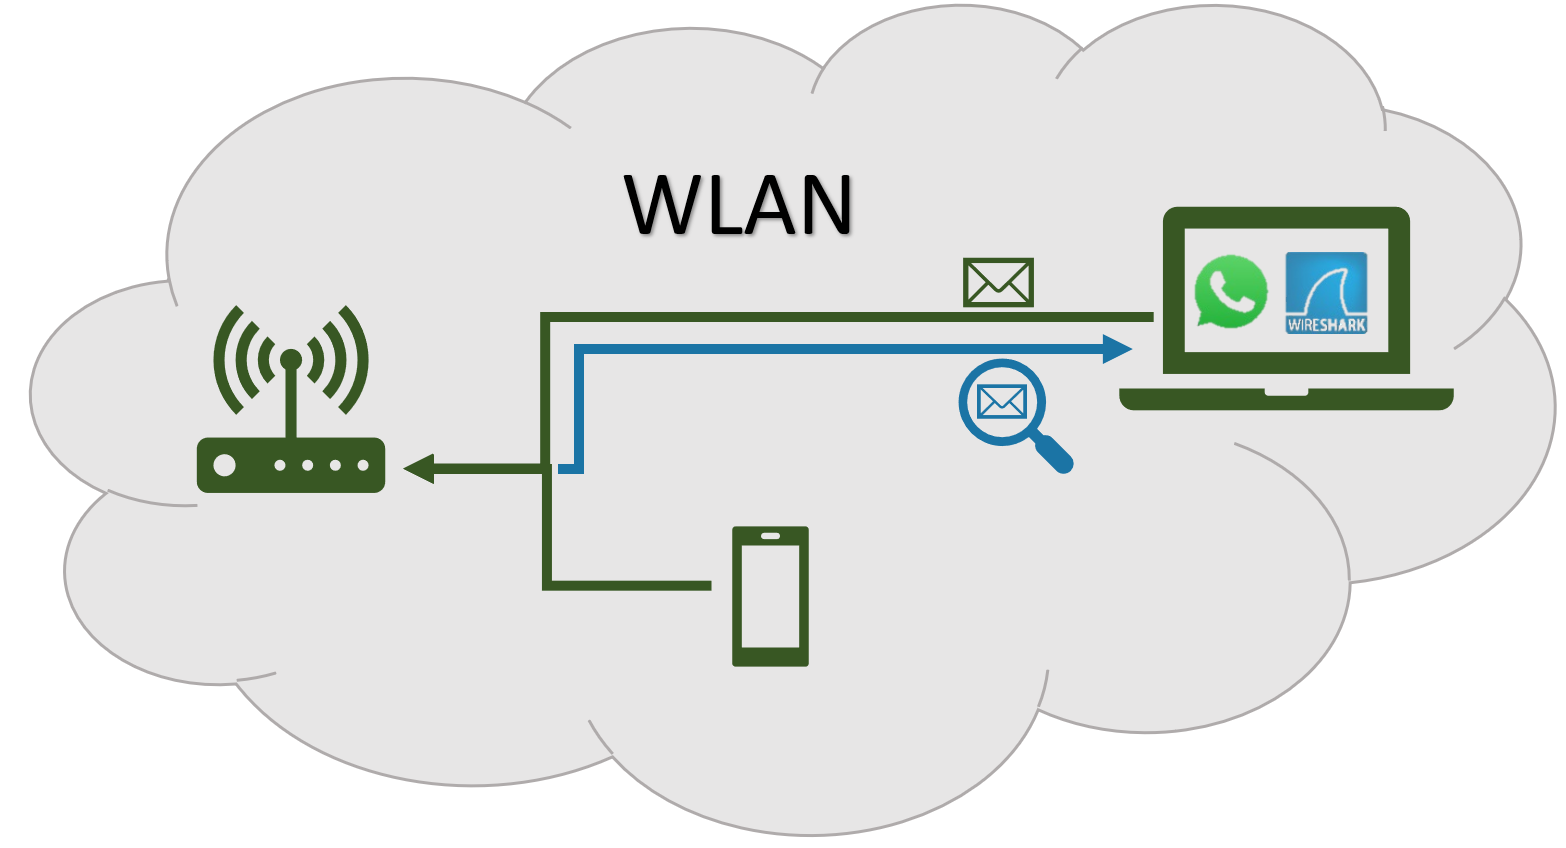
\includegraphics[width=9cm]{Aufbau}
\end{center}

\begin{description}
    \item \textbf{Laptop}
        \begin{description}
            \item \textit{WebWhatsApp}: 
                Über diesen Laptop wird WebWhatsApp aufgerufen. Der Client ist 
                bereits auf registriert. 
            \item \textit{Wireshark}:
                Zusätzlich ist Wireshark installiert um die gesamte Netzwerkkommunikation
                zu analysieren.
        \end{description}
    \item \textbf{Smartphone}
    \begin{description}
       \item Das Smartphone über das der Laptop Client bei WhatsApp registriert ist, muss
            sich im Internet befinden. In diesem Fall ist es im gleichen WLAN (müsste es aber nicht sein). 
    \end{description};
\end{description};

\subsection{Analyse mit Wireshark}
\subsubsection{Vorgehen und erster Überblick}
\subsubsection{TCP Handshake}
\subsubsection{Einigen auf Cipher-Suite}
\subsubsection{Übertragung der Application Data}